The camera used in this project is the Logitech Quickcam Orbit MP webcam. The specifications are:

\begin{itemize}
\setlength{\itemsep}{0mm}
	\item Native image resolution: 1280 x 960.
	\item Still-image capture resolution: 1280 x 960.
	\item Video capture resolution: 960 x 720.
	\item Framerate: 30 fps.
	\item Connection: USB.
\end{itemize}.

The camera parameter settings can be altered in the Logitech QuickCam software. There are many different parameters and the default settings produce the image seen in figure \ref{fig:defaultcamera}.

\begin{figure}[htpb]
\begin{center}
\leavevmode
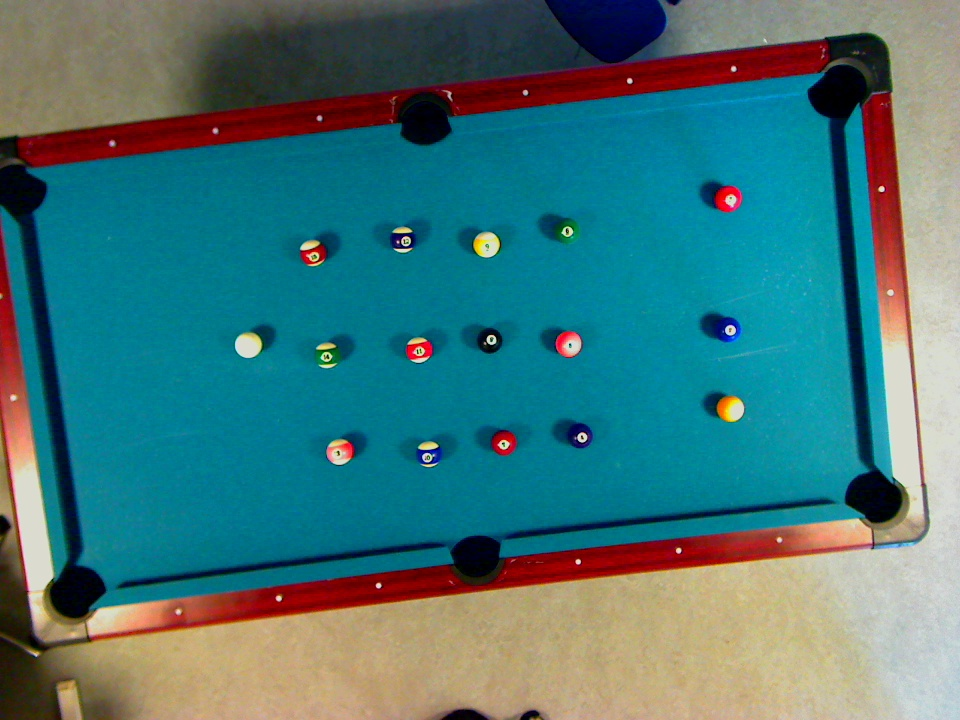
\includegraphics[width=0.5\textwidth]{images/default}
\end{center}
\caption{Default settings of camera parameters.}
\label{fig:defaultcamera}
\end{figure} 
	
As seen in figure \ref{fig:defaultcamera} the ball towards the lower right corner is the solid yellow, but it seems to be half yellow and half white. This is due to overexposure and therefore saturation of the bright colors. The default camera settings are not the optimal settings for this project.	

A few examples of wrong settings can be seen in figure \ref{fig:wrongcamera} . They are divided into settings that only occur in software and settings where hardware parameters have been altered.

\begin{figure}[htpb]
\centering
\subfloat[Software: Wrong whitebalance.]
{
	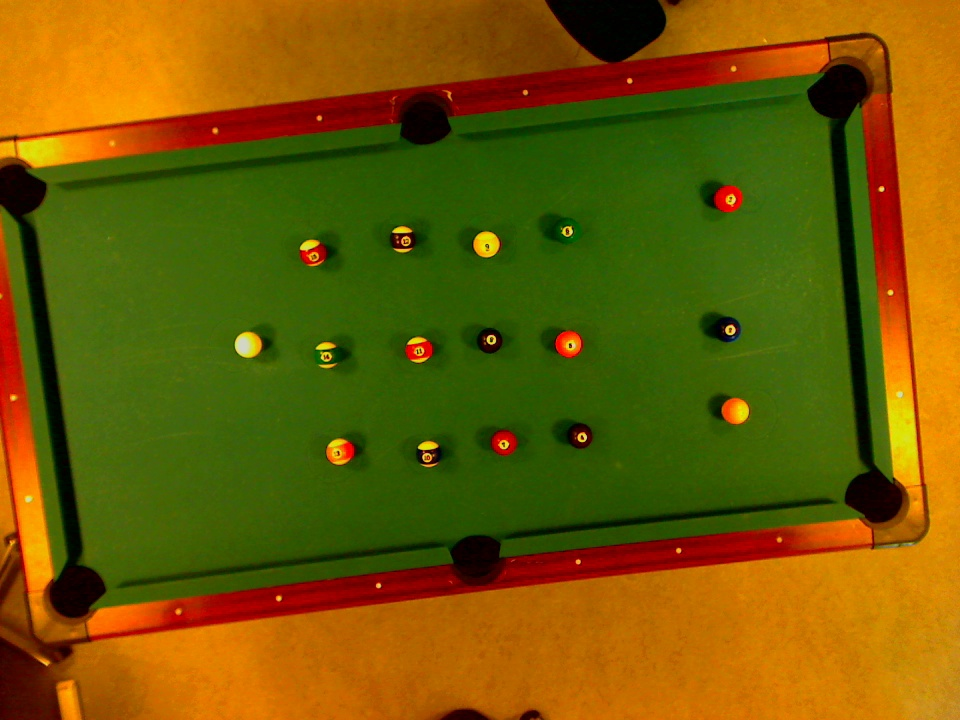
\includegraphics[width=0.4\textwidth]{images/badwhite}
}
\subfloat[Hardware: Extreme saturation.]
{
	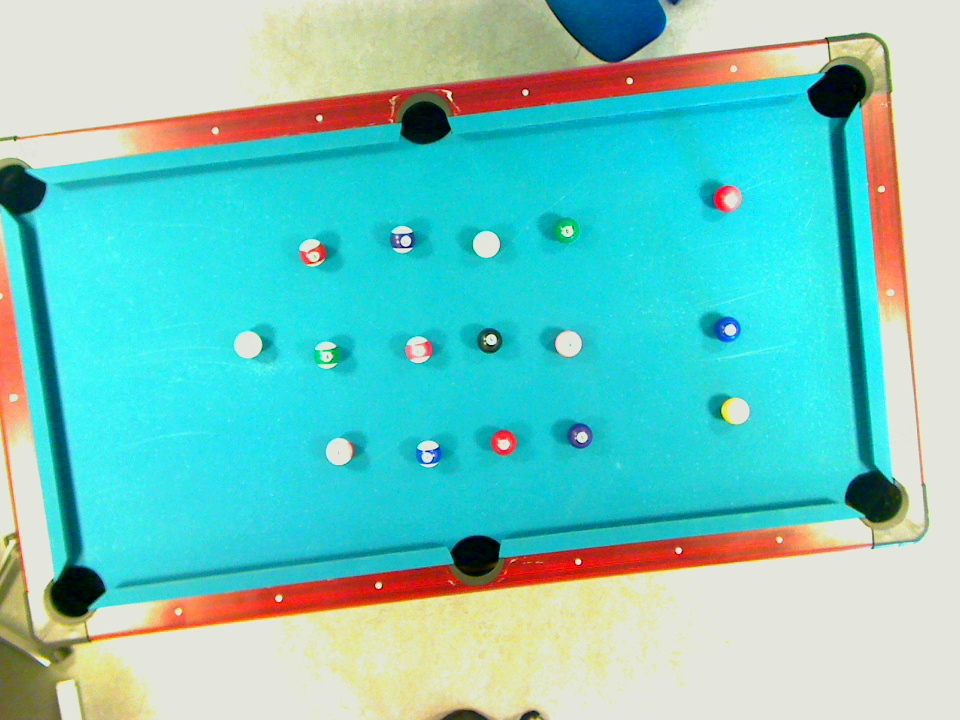
\includegraphics[width=0.4\textwidth]{images/overexposure}
}\\
\subfloat[Hardware: Camera out of focus.]
{
	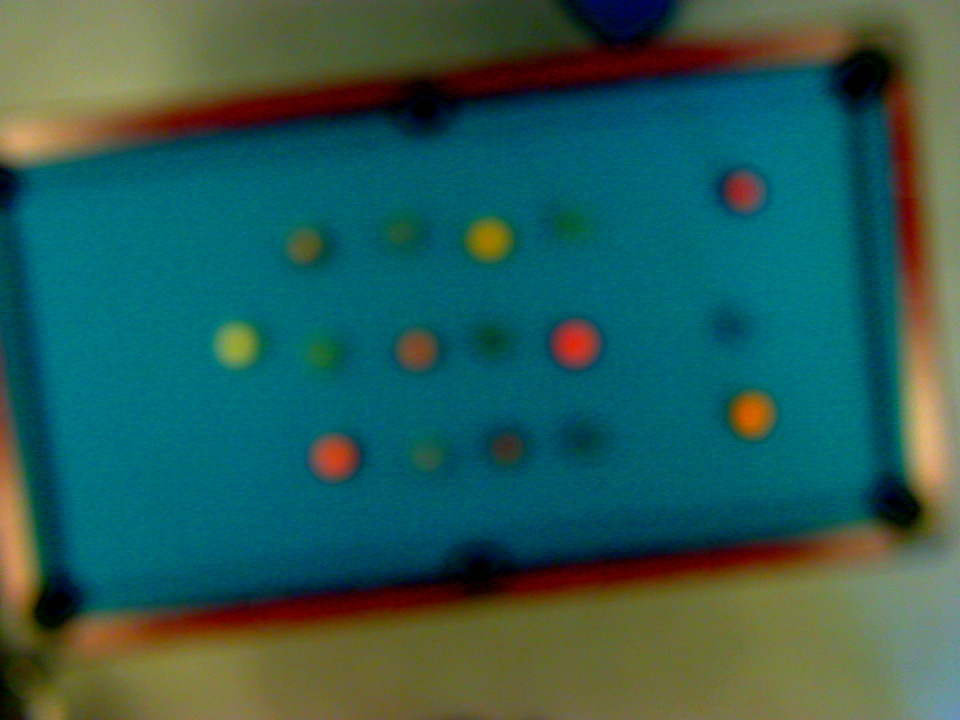
\includegraphics[width=0.4\textwidth]{images/nofocus}
}
\subfloat[Conditions/Hardware: Low saturation or too dark environment.]
{
	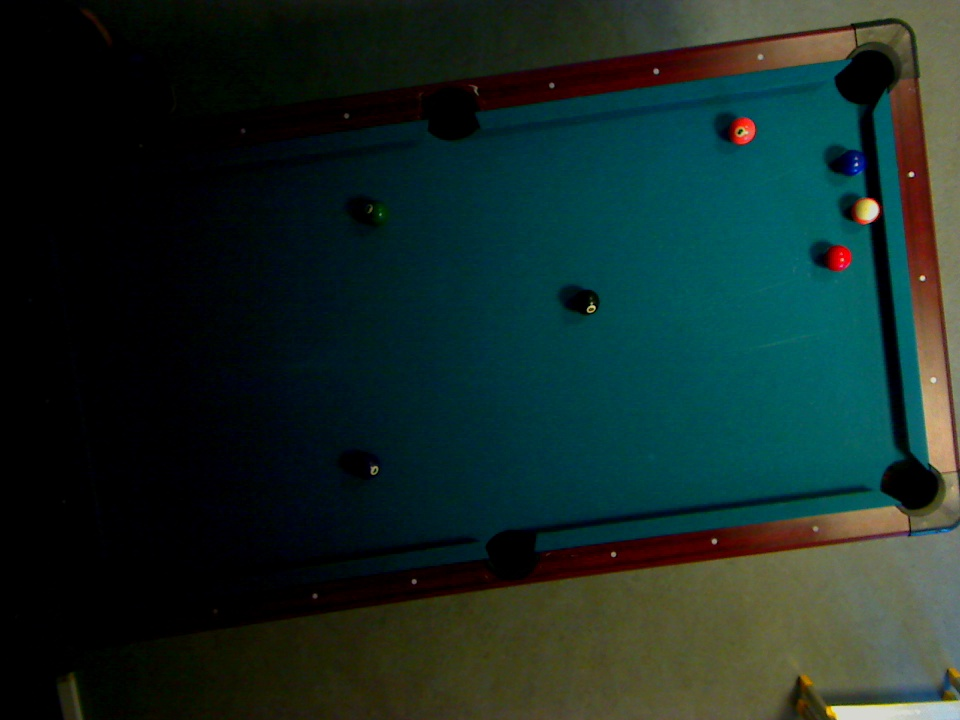
\includegraphics[width=0.4\textwidth]{images/toodark}
}

\caption{Examples of camera setting.}
\label{fig:wrongcamera}
\end{figure} 

The optimal settings can only be set using Logitech Quickcam software with user input. The best image achieved can be seen in figure \ref{fig:bestimgcamera}. The balls are easily distinguishable from each other and no saturation occurs.

\begin{figure}[htpb]
\begin{center}
\leavevmode
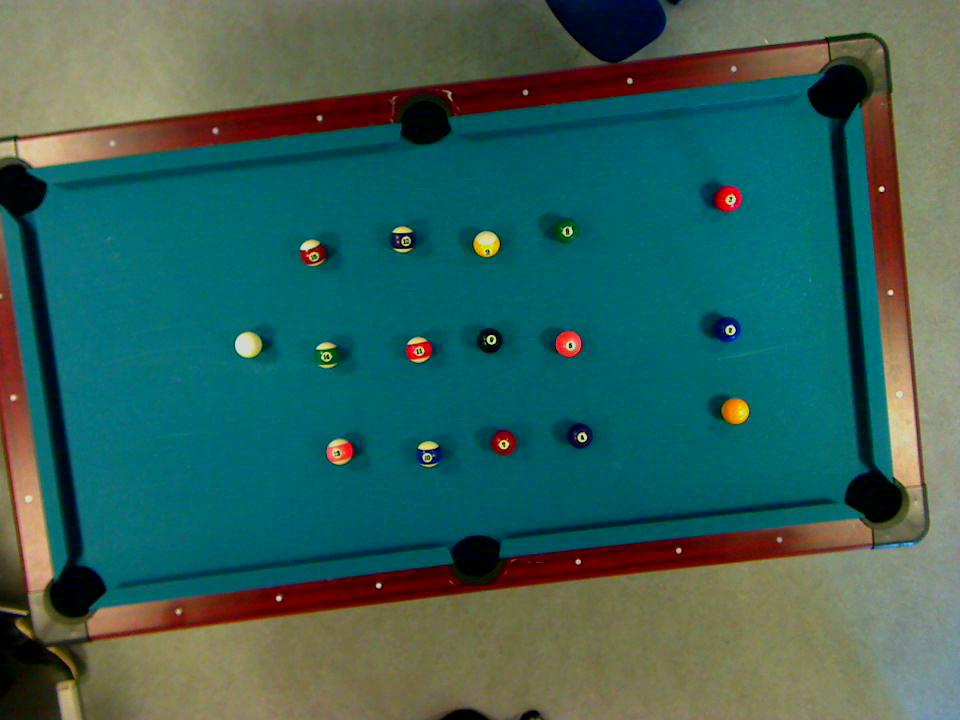
\includegraphics[width=0.5\textwidth]{images/good-from-program}
\end{center}
\caption{Image using optimal settings.}
\label{fig:bestimgcamera}
\end{figure} 

It is very important that the settings are set correctly to produce an optimal image. If the image is too saturated, a bright solid ball could appear as a ball with striped color. If the color balance is not optimal the red, orange and brown balls might also look very alike.